\subsection{High Level Message Sequence Chart}
	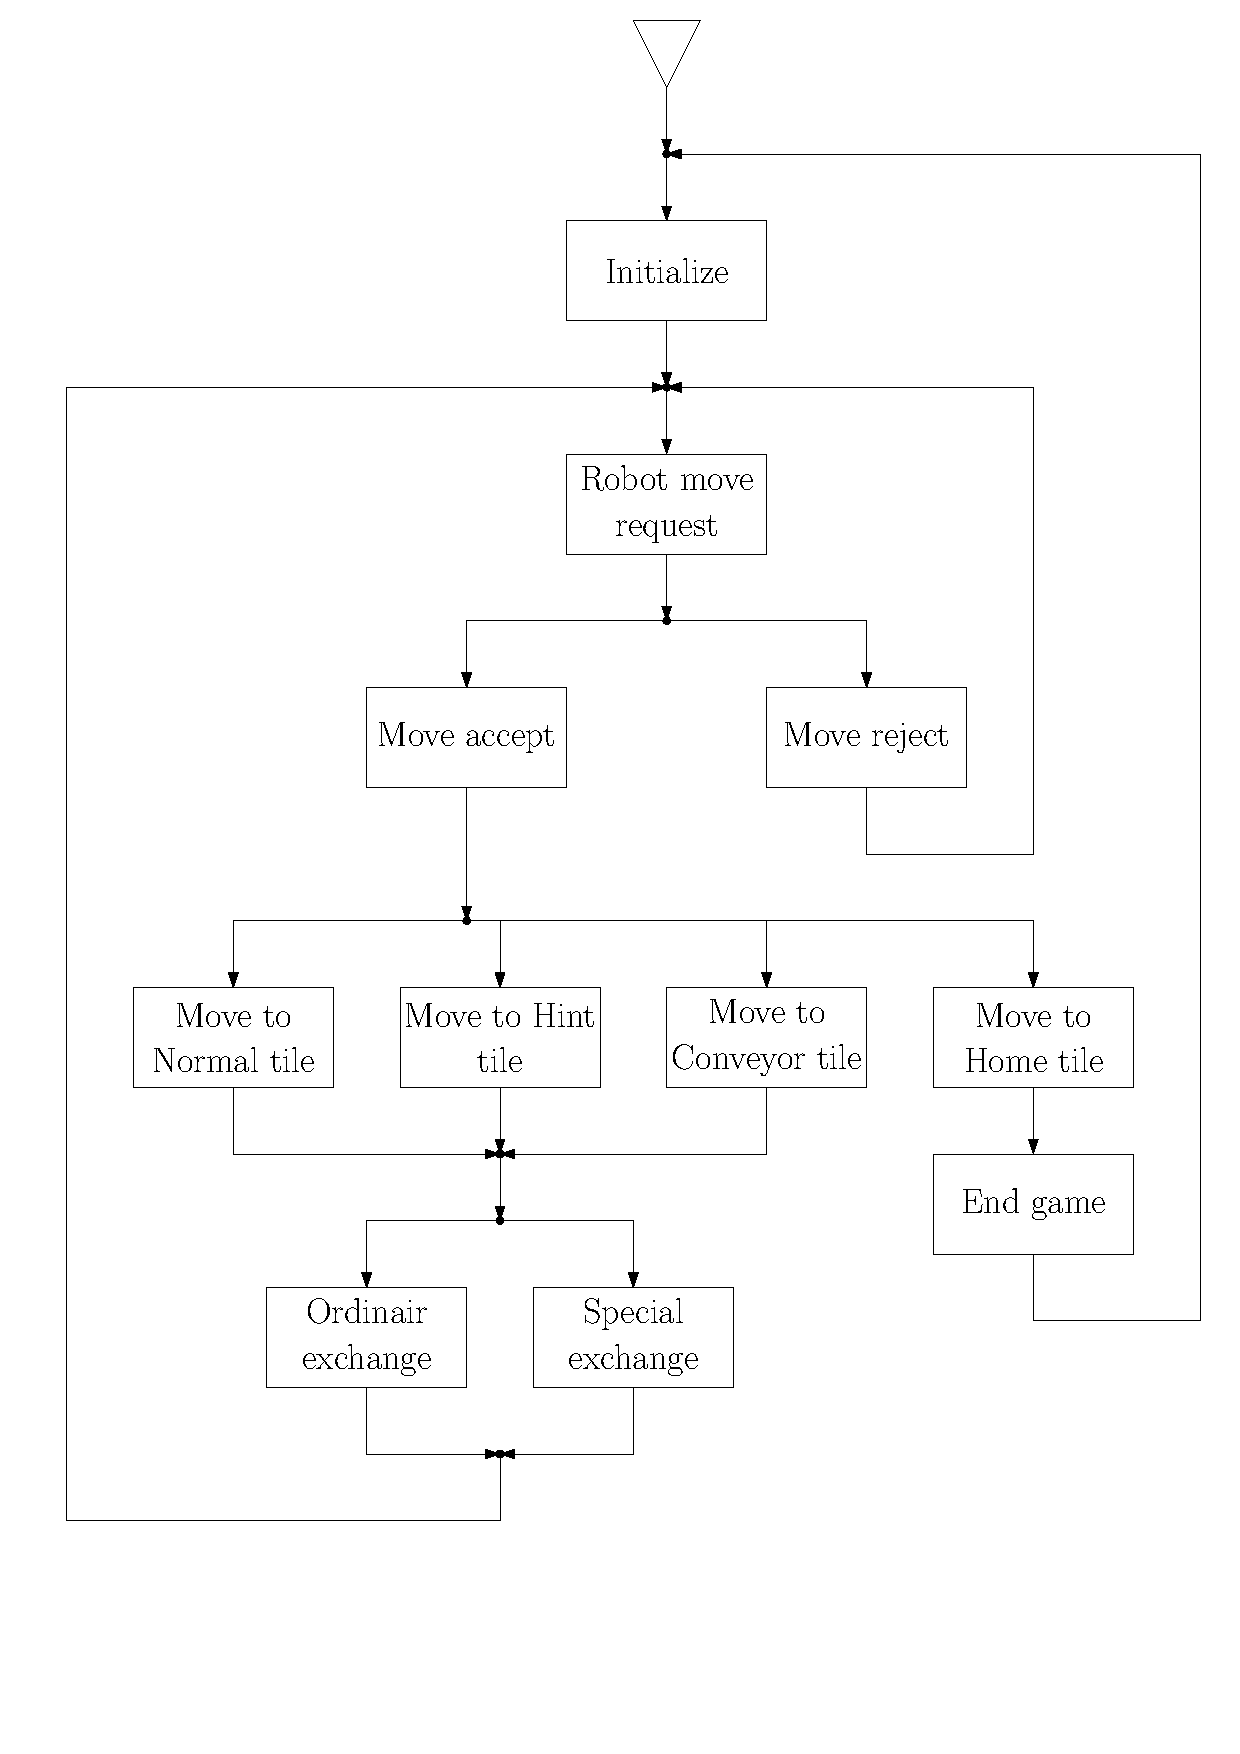
\includegraphics[width=\linewidth,bb=0 0 680 1000]{MSC-files/HMSC.pdf}
	
\subsection{Message Sequence Charts}
	\subsubsection{Robot move - OK}
	\begin{msc}
		msc
		{

		a [label="Robot type A"],
		b [label="Robot type B"],
		c [label="Controller"],
		d [label="Board"];

		a box a [label=""],
		b box b [label=""],
		c box c [label=""],
		d box d [label=""];

		|||;

		a -> c [label="Move request"];
		c => d [label="Move OK?"];
		d >> c [label="OK"];
		c => d [label="Make move"];
		d box d [label="Save location of robot"];
		d >> c [label="OK"];
		c -> a [label="OK"];

		|||;

		---;

		|||;

		b -> c [label="Move request"];
		c => d [label="Move OK?"];
		d >> c [label="OK"];
		c => d [label="Make move"];
		d box d [label="Save location of robot"];
		d >> c [label="OK"];
		c -> b [label="OK"];

		|||;

		a box a [label="", textbgcolor="black"],
		b box b [label="", textbgcolor="black"],
		c box c [label="", textbgcolor="black"],
		d box d [label="", textbgcolor="black"];

		}
	\end{msc}
	
	\subsubsection{Robot move - Not OK}
	\begin{msc}
msc
{

a [label="Robot"],
c [label="Controller"],
d [label="Board"],
r [label="Rule"];

a box a [label=""],
c box c [label=""],
d box d [label=""],
r box r [label=""];

|||;

a -> c [label="Move request"];
c => d [label="Move OK?"];
d => r [label="Move OK?"];
r >> d [label="NOK"];
d >> c [label="NOK"];
c -> a [label="NOK"];

|||;

a box a [label="", textbgcolor="black"],
c box c [label="", textbgcolor="black"],
d box d [label="", textbgcolor="black"],
r box r [label="", textbgcolor="black"];

}
\end{msc}

	
	\subsubsection{Robot move - Hint tile}
	\begin{msc}
msc
{

a [label="Robot type A"],
b [label="Robot type B"],
c [label="Controller"],
d [label="Board"];

a box a [label=""],
b box b [label=""],
c box c [label=""],
d box d [label=""];

|||;

a -> c [label="Move request"];
c => d [label="Move OK?"];
d >> c [label="OK"];
c => d [label="Make move"];
d rbox d [label="Save location of robot"];
d >> c [label="Hinttile"];
c => d [label="Get Hint"];
d rbox d [label="Generate hint"];
d >> c [label="Hint"];
c -> a [label="Hint"];

|||;

---;

|||;

b -> c [label="Move request"];
c => d [label="Move OK?"];
d >> c [label="OK"];
c => d [label="Make move"];
d rbox d [label="Save location of robot"];
d >> c [label="Hinttile"];
c => d [label="Get Hint"];
d rbox d [label="Generate hint"];
d >> c [label="Hint"];
c -> b [label="Hint"];

|||;

a box a [label="", textbgcolor="black"],
b box b [label="", textbgcolor="black"],
c box c [label="", textbgcolor="black"],
d box d [label="", textbgcolor="black"];

}
\end{msc}

	
	\subsubsection{Robot move - Conveyor Belt}
	\begin{msc}
msc
{

a [label="Robot"],
c [label="Controller"],
d [label="Board"],
r [label="Rule"];

a box a [label=""],
c box c [label=""],
d box d [label=""],
r box r [label=""];

|||;

a -> c [label="Move request"];
c => d [label="Move OK?"];
d => r [label="Move OK?"];
r >> d [label="OK"];
d >> c [label="OK"];
c => d [label="Make move"];
d >> c [label="OK"];
c => d [label="Make move"];
d >> c [label="Conveyer belt"];
c -> a [label="Conveyer belt"];

|||;

a box a [label="", textbgcolor="black"],
c box c [label="", textbgcolor="black"],
d box d [label="", textbgcolor="black"],
r box r [label="", textbgcolor="black"];

}
\end{msc}

	
	\subsubsection{Robot move - Home tile}
	\begin{msc}
msc
{

a [label="Robot type A"],
b [label="Robot type B"],
c [label="Controller"],
d [label="Board"];

a box a [label=""],
b box b [label=""],
c box c [label=""],
d box d [label=""];

|||;

a -> c [label="Move request"];
c => d [label="Move OK?"];
d >> c [label="OK"];
c => d [label="Make move"];
d rbox d [label="Save location of robot"];
d rbox d [label="Save which robot wins"];
d >> c [label="WIN"];
c -> a [label="WIN"];
d rbox d [label="Destroy rest"];

|||;

---;

|||;

b -> c [label="Move request"];
c => d [label="Move OK?"];
d >> c [label="OK"];
c => d [label="Make move"];
d rbox d [label="Save location of robot"];
d rbox d [label="Save which robot wins"];
d >> c [label="WIN"];
c -> b [label="WIN"];
d rbox d [label="Destroy rest"];

|||;

a box a [label="", textbgcolor="black"],
b box b [label="", textbgcolor="black"],
c box c [label="", textbgcolor="black"],
d box d [label="", textbgcolor="black"];

}
\end{msc}

	
	\subsubsection{Tiles exchange}
	\begin{msc}
msc
{

b [label="Board"],
c [label="Controller"];

c box c [label=""],
b box b [label=""];

|||;

c=>b [label="requestTilesExchange()"];
b rbox b [label="exchange two tiles"];
b>>c [label="empty RobotPair"];

|||;

b box b [label="",textbgcolor="black"],
c box c [label="",textbgcolor="black"];

}
\end{msc}
\digraph[scale=0.5]{HMSC_exch}{
rankdir=LR;
p2 [label="",shape="point"];
p5 [label="",shape="point"];
p6 [label="",shape="point"];
p7 [label="",shape="point"];
init [label="Initialize",shape="Mrecord"];
mvreq [label="Robot move request",shape="Mrecord"];
retnt [label="Return Normal tile",shape="Mrecord"];
retht [label="Return Hint tile",shape="Mrecord"];
retct [label="Return Conveyor tile",shape="Mrecord"];
ordex [label="Ordinary exchange",shape="Mrecord",style=filled];
init->p2;
p2->mvreq;
retnt->p5;
retht->p5;
retct->p5;
p5->p6;
p6->ordex;
ordex->p7;
p7->p2;
}

	
	\subsubsection{Tiles exchange special}
	\begin{msc}
msc
{

b [label="Board"],
c [label="Controller"],
p1 [label="Robot1"],
p2 [label="Robot2"],
v [label="Viewer"];

c box c [label=""],
b box b [label=""],
p1 box p1 [label=""],
p2 box p2 [label=""],
v box v [label=""];

|||;
c=>b [label="requestTilesExchange()"];
b rbox b [label="getValidTiles()"];
b rbox b [label="exchange two valid tiles"];
b rbox b [label="rotate robot1 and rotate tiles"];
b>>c [label="RobotPair with one robot"];
...;
c->p1 [label="notifyAutoMovement()"];
c -> v [label="notifyStateChange()"];
...;

|||;

b box b [label="",textbgcolor="black"],
c box c [label="",textbgcolor="black"],
p1 box p1 [label="",textbgcolor="black"],
p2 box p2 [label="",textbgcolor="black"],
v box v [label="",textbgcolor="black"];

}
\end{msc}

\digraph[scale=0.5]{HMSC_exchsp}{
rankdir=LR;
p2 [label="",shape="point"];
p5 [label="",shape="point"];
p6 [label="",shape="point"];
p7 [label="",shape="point"];
p22 [label="",shape="point"];
p77 [label="",shape="point"];
notrob2 [label="Notify robots",shape="Mrecord"];
init [label="Initialize",shape="Mrecord"];
mvreq [label="Robot move request",shape="Mrecord"];
retnt [label="Return Normal tile",shape="Mrecord"];
retht [label="Return Hint tile",shape="Mrecord"];
retct [label="Return Conveyor tile",shape="Mrecord"];
spcex [label="Special exchange",shape="Mrecord",style=filled];
init->p2;
p2->mvreq;
retnt->p5;
retht->p5;
retct->p5;
p5->p6;
p6->spcex;
spcex->p7;
p7->p77;
p77->p22;
p22->p2;
p77->notrob2;
notrob2->p22;
}

	